% withpage: ページ番号をつける (著者確認用)
% english: 英語原稿用フォーマット
\documentclass{ipsjprosym}
%\documentclass[withpage,english]{ipsjprosym}

\usepackage[dvipdfmx]{graphicx}
\usepackage{latexsym}

\usepackage{listings}

\begin{document}

% Title, Author %%%%%%%%%%%%%%%%%%%%%%%%%%%%%%%%%
\title{環境にメソッドを直接格納する \\ 新しいオブジェクトシステムの提案}

\affiliate{COINS}{筑波大学情報学群情報科学類}
\affiliate{CS}{筑波大学システム情報系}

\author{林 拓人}{Takuto Hayashi}{COINS}[hayashi@ialab.cs.tsukuba.ac.jp]
\author{前田 敦司}{Atusi Maeda}{CS}[maeda@cs.tsukuba.ac.jp]

\begin{abstract}
%[概要(400字程度)]
従来のクラスベース・オブジェクトシステムは,メソッドをクラスに格納するものと総称関数に格納するもの
(メソッドがクラスに属すものと総称関数に属すもの)とに分けられる.
本論文はこれらのいずれとも異なり,環境にメソッドを直接格納する新しいオブジェクトシステムを
提案する.
クラスや総称関数と言った枠を廃し,クラス名とメソッド名の組をキーとして環境にメソッドを直接格納する.
これにより変数に対して行えるあらゆる操作がメソッドに対しても行えるようになり,従来の方式に比べ
シンプルな仕組みでより柔軟なオブジェクト指向プログラミングが可能となる.
提案する手法の有用性を実証するため,このオブジェクトシステムを搭載する独自言語Suzuの
処理系を実装した.
これが実際に言語内DSL(Domain Specific Language)の作成に有用であることを示す.
従来のオブジェクトシステムにおける類似した概念等との関連についても議論する.
\end{abstract}

\begin{jkeyword}
オブジェクトシステム,メソッド,クラス,総称関数,環境
\end{jkeyword}

\maketitle

% Body %%%%%%%%%%%%%%%%%%%%%%%%%%%%%%%%%
\section{序論}

従来のクラスベース・オブジェクトシステムは,メソッドの格納方式に着目してモデル化すると
次の2つのモデルに分類することができる.
1つはクラスにメソッドを格納するモデル,もう1つはCLOS\cite{Ida:2010}のように
総称関数にメソッドを格納するモデルである.

本論文は,これら2つの格納モデルに対する分析に基づき考案した,全く新しい格納モデルを持つ
オブジェクトシステムを提案する.
また,その特徴を最大限に生かせるよう独自に設計したプログラミング言語Suzuを用いて,提案する
オブジェクトシステムの評価を行う.

\section{従来のオブジェクトシステム}

ここではモデルを単純化するため,単一ディスパッチについてのみ考える.
多重ディスパッチへのモデルの拡張については\ref{sec:multiple-dispatch}節で検討する.

\subsection{クラスにメソッドを格納するモデル}

クラスにメソッドを格納するモデルでは環境にクラスを格納し,クラスにメソッドを格納する
(図\ref{fig:classes}).
ここで環境はクラス名をキーとしてクラスを格納する辞書であり,クラスはメソッド名をキーとして
メソッドを格納する辞書である.
SmalltalkやRubyなどのオブジェクトシステムはこのモデルに分類される.

\subsection{総称関数にメソッドを格納するモデル}
\label{sec:generic-finctions}

総称関数にメソッドを格納するモデルでは環境に総称関数を格納し,総称関数にメソッドを格納する
(図\ref{fig:generic-functions}).
ここで環境はメソッド名をキーとして総称関数を格納する辞書であり,総称関数はクラス名をキーとして
メソッドを格納する辞書である.
単一ディスパッチに限定したCLOSはこのモデルに分類される.

\section{提案するオブジェクトシステム}
\label{sec:proposal}

従来のオブジェクトシステムの分類先である2つのモデルは,どちらもクラス名とメソッド名が決まれば
メソッドが一意に定まるという特徴を持つ.
また,環境という辞書の中にクラスあるいは総称関数という辞書が入れ子になっている構造も
共通している.

提案するオブジェクトシステムはこのようなクラスや総称関数による入れ子構造を廃し,
\textbf{環境にメソッドを直接格納するモデル}を採用する(図\ref{fig:environment}).
ここで環境は\textbf{クラス名とメソッド名の組}をキーとしてメソッドを格納する辞書である.

このモデルの特徴は,メソッドの格納方式が一般的な変数の格納方式と類似していることである.
メソッドがクラス名とメソッド名の組をキーとして環境に格納されるのに対し,変数は変数名を
キーとして環境に格納される.

これはすなわち,「変数名」を「クラス名とメソッド名の組」に置き換えることで,
\textbf{変数に対して行えるあらゆる操作がメソッドに対しても行えるようになる}ということである.
具体的には,ブロック単位でのスコープの制御やシャドーイング,モジュールからのエクスポート・
インポート,仮引数やパターンマッチングのパターンとしての指定などが挙げられる.
\ref{sec:implementation}節では提案するオブジェクトシステムを搭載した独自の
プログラミング言語Suzuを用いて,この特徴を生かした実際のプログラム例を示す.

\begin{figure}
\centering
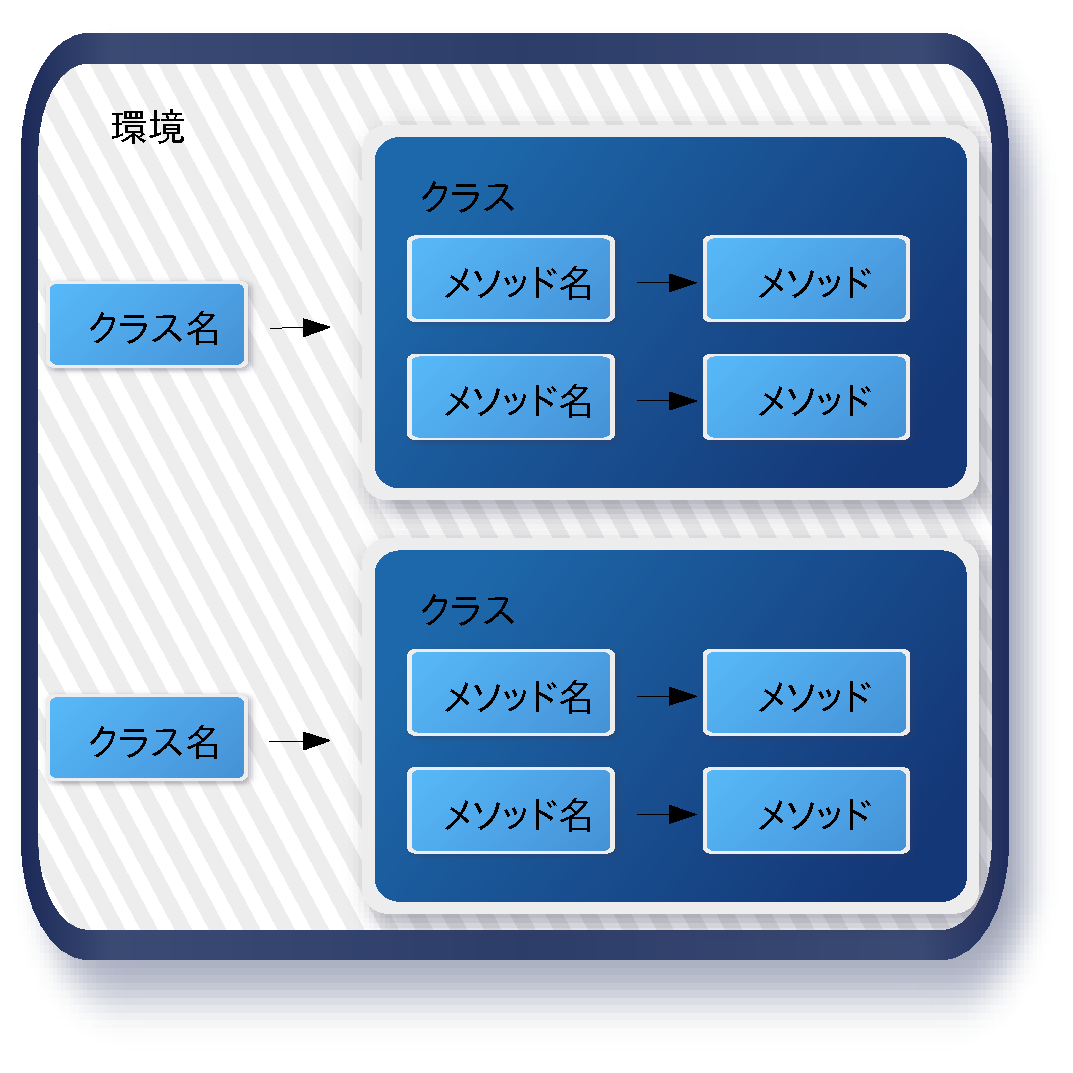
\includegraphics[width=7cm]{fig/classes-crop.pdf}
\caption{クラスにメソッドを格納するモデル}
\label{fig:classes}
\end{figure}

\begin{figure}
\centering
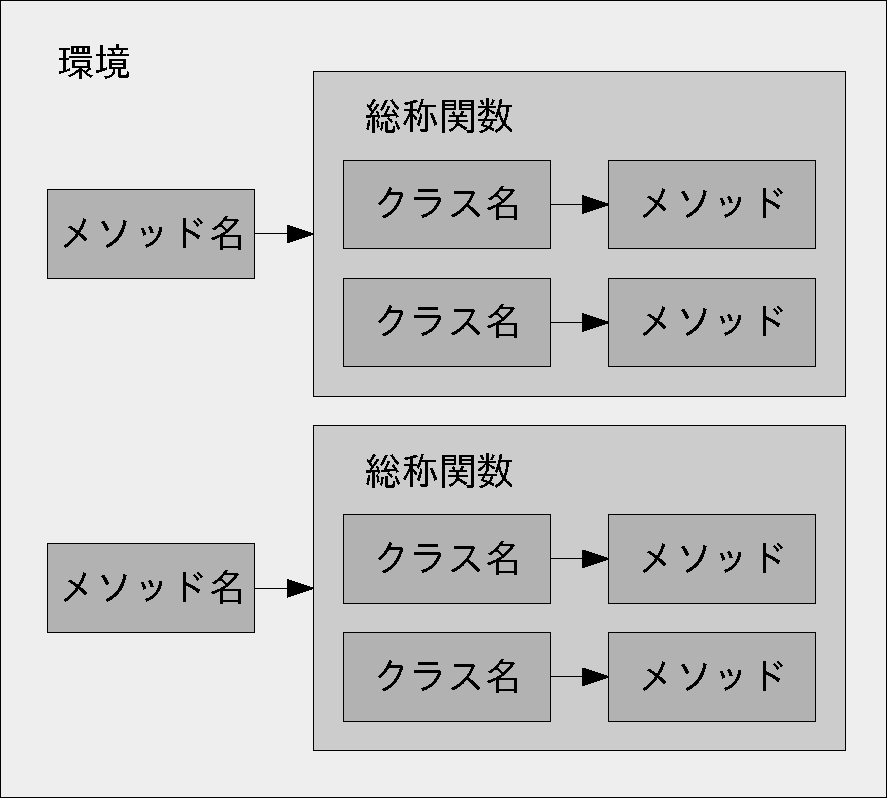
\includegraphics[width=7cm]{fig/generic-functions-crop.pdf}
\caption{総称関数にメソッドを格納するモデル}
\label{fig:generic-functions}
\end{figure}

\begin{figure}
\centering
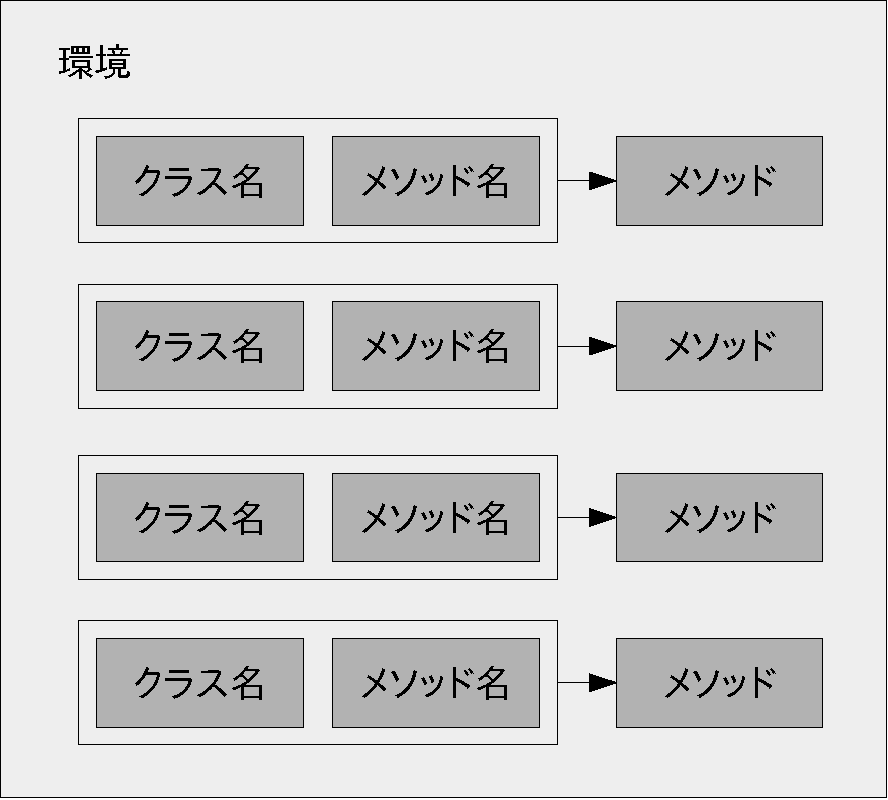
\includegraphics[width=7cm]{fig/environment-crop.pdf}
\caption{環境にメソッドを直接格納するモデル}
\label{fig:environment}
\end{figure}

\section{実装:プログラミング言語Suzu}
\label{sec:implementation}

環境にメソッドを直接格納するモデルに基づき設計した独自のプログラミング言語Suzuの解説とその
プログラム例により,提案するオブジェクトシステムの有用性を示す.
処理系のソースコードはGitリポジトリ(https://github.com/takuto-h/suzu)にて公開している.

\subsection{Suzuの概要}

クラス定義は以下のようにして行う.
\begin{quote}
\begin{verbatim}
class Vector = make_vector:
  x
  y
end
\end{verbatim}
\end{quote}
これにより,フィールド\verb|x|,\verb|y|を持つクラス\verb|Vector|と
コンストラクタ関数\verb|make_vector|,ゲッターメソッド\verb|Vector#x|,
\verb|Vector#y|が定義される.
\verb|<class-name>#<method-name>|というのは\ref{sec:proposal}節で述べた
クラス名とメソッド名の組であり,Suzuにおけるメソッドの参照構文でもある.

インスタンス化してメソッドを呼び出すには以下のようにする.
なお,\verb|write_line|はCの\verb|printf|に相当する書式付き出力関数,\verb|//|以降は
コメントである.
\begin{quote}
\begin{verbatim}
let a = make_vector(1, 2)
write_line("{0}, {1}", a.x, a.y)
  //=> 1, 2
\end{verbatim}
\end{quote}
関数\verb|make_vector|を呼び出して\verb|Vector|のインスタンスを生成し,
変数\verb|a|に代入している.
コンストラクタ関数はフィールドを宣言された順に与えられた引数で初期化する.
メソッド呼び出し\verb|a.x|によってメソッド\verb|Vector#x|が呼び出され,
フィールド\verb|x|の値が返り,\verb|1|が出力される.
同様に\verb|y|の値\verb|2|も出力される.

メソッドは以下のように定義する.
\begin{quote}
\begin{verbatim}
def Vector#add(self, other):
  make_vector(self.x + other.x,
              self.y + other.y)
end
let b = make_vector(3, 4)
let c = a.add(b)
write_line("{0}, {1}", c.x, c.y)
  //=> 4, 6 
\end{verbatim}
\end{quote}
メソッド\verb|Vector#add|を定義した.\verb|a.add(b)|というメソッド呼び出しでは
\verb|self|に\verb|a|の値が,\verb|other|に\verb|b|の値が代入される.

Suzuではユーザーが独自の演算子をメソッドとして定義できる.
\begin{quote}
\begin{verbatim}
let Vector#(+) = Vector#add
let d = b + c
write_line("{0}, {1}", d.x, d.y)
  //=> 7, 10
\end{verbatim}
\end{quote}

Suzuのオブジェクトシステムは環境にメソッドを格納するため,ローカル環境にメソッドを定義する
ことが可能だ.
ここで言うローカル環境とは,ブロック(制御構文でインデントを行う部分),関数,
モジュールといったあらゆる局所的なスコープのことである.
\begin{quote}
\begin{verbatim}
def Vector#m(self):
  write_line("global")
end
begin:
  def Vector#m(self):
    write_line("local")
  end
  d.m  //=> local
end
d.m  //=> global
\end{verbatim}
\end{quote}

Suzuのモジュールは,他の言語における変数のようにメソッドを個別にエクスポートできる.
\begin{quote}
\begin{verbatim}
module A:
  class C = ...
    ...
  end
  def f(...):
    ...
  end
  def C#m(...):
    ...
  end
  def C#n(...):
    ...
  end
  export f, C#m
end
\end{verbatim}
\end{quote}
上の例ではモジュール\verb|A|は関数\verb|f|とメソッド\verb|C#m|をエクスポートするが,
\verb|C#n|はエクスポートしない.エクスポートされた変数を参照するには\verb|A::f|のようにする.

モジュールは局所的に\verb|open|することができる.
モジュールを\verb|open|するとエクスポートされている変数やメソッドがそのスコープで
直接定義されたようにインポートすることができる.
また,\verb|except|キーワードを用いてインポートの対象から除外することもできる.
\begin{quote}
\begin{verbatim}
module B:
  ...
  export f, g, C, C#m, C#n
end
begin:
  open B except g, C#n
  ...
end
\end{verbatim}
\end{quote}
上の例では\verb|begin|から\verb|end|までのスコープへ,
モジュール\verb|B|でエクスポートされているもののうち\verb|g|と\verb|C#n|を除いて
インポートを行う.

Suzuは継承機構を持たず,実装の再利用はTraits\cite{Scharli:2003}を用いて行う.
ただし,SuzuのTraitはそのオブジェクトシステムに適合するよう他の言語と比べて多少
趣の異なるものとなっている.
\begin{quote}
\begin{verbatim}
trait T(C, C#m, C#n):
  def C#o(self, ...):
    ...
    self.m(...)
    ...
  end
  def C#p(self, ...):
    ...
    self.n(...)
    ...
  end
  export C#o, C#p
end
\end{verbatim}
\end{quote}
Traitは\textbf{クラスやメソッドを受け取ってモジュールを返す関数}として表現される.
使用する側は以下のようにする.
\begin{quote}
\begin{verbatim}
open T(D, D#m, D#n)
open T(E, E#m, E#n)
\end{verbatim}
\end{quote}
これにより,\verb|D#o|,\verb|D#p|,\verb|E#o|,\verb|E#p|が定義される.
Trait同士の加算は単に\verb|open|を並べればよい.メソッドの減算は\verb|except|を用いる.
メソッドのリネームは\verb|except|に\verb|let|を用いた個別のインポートを組み合わせる.
例えばTrait \verb|S|によって定義されるメソッド\verb|m|を\verb|n|にリネームしたい場合,
以下のようにする.
\begin{quote}
\begin{verbatim}
open S(C) except C#m
let C#n = S(C)::(C#m)
\end{verbatim}
\end{quote}

\subsection{プログラム例:PEGパーザコンビネータ}

Suzuの有用性を示す例として,PEGパーザコンビネータライブラリを作成した.
ソースコードは付録として\ref{sec:peg-source}節に記載している.

このライブラリを用いると,パーザを言語内DSLとして簡単に記述することができる.
例えば,言語$\{a^n b^n c^n:n\ge1\}$のパーザは以下のようにして書ける.
なお\verb|p|はデバッグ用の出力関数である.

\begin{quote}
\begin{verbatim}
let s = begin:
  open PEG::New()
  "S" <- and(nt_ref("A") &+
             not(char('b')))
      &+ one_or_more(char('a'))
      &+ nt_ref("B")
      &+ not(char('c'))
  "A" <- char('a')
      &+ zero_or_one(nt_ref("A"))
      &+ char('b')
  "B" <- char('b')
      &+ zero_or_one(nt_ref("B"))
      &+ char('c')
  nt_ref("S")
end
p(PEG::parse(s, ""))
  //=> Failure()
p(PEG::parse(s, "abc"))
  //=> Success(...)
p(PEG::parse(s, "ab"))
  //=> Failure()
p(PEG::parse(s, "aaabbbccc"))
  //=> Success(...)
p(PEG::parse(s, "aabbbccc"))
  //=> Failure()
\end{verbatim}
\end{quote}

パーザを定義する際はまず新しいスコープで\verb|PEG::New|を呼び出し\verb|open|する.
これによりコンビネータ関数やメソッドがインポートされる.
例えば\verb|nt_ref|は非終端記号を参照するコンビネータである.

\verb|String#(<-)|は新しい非終端記号を定義する演算子であり.既存の
\verb|String|クラスにこのスコープでのみ有効な新たなメソッドとして定義されている.
このように,Suzuのオブジェクトシステムは特定のスコープでのみ有効なメソッドを定義
できることで,モジュラリティの高い言語内DSLの作成を容易にしている.

\section{関連研究}

Suzuのオブジェクトシステムについて,従来のオブジェクトシステムに対しこれと似た柔軟性を
与えようとする取り組みや,構造上の類似性を持つ概念との比較を行う.

\subsection{ContextJ}

ContextJ\cite{AppeltauerMalte:2011}は,文脈指向プログラミングにおけるlayerという
概念に基づいたJavaの拡張言語である.
layerを切り替えるによりメソッドの定義を切り替えることができる.

layerは重ねられるという点でSuzuの環境と類似している.しかしながら,メソッドの定義が
クラスの内部でしか行えないという点で柔軟性に欠ける.

\subsection{GluonJ}

GluonJ\cite{Chiba:2010:MMC:1869459.1869503}は,Javaでアスペクト指向
プログラミングを行うためのシステムである.
Glueと呼ばれるクラスを定義することによって,既存のクラスについてメソッドを再定義することが
できる.

クラスの外部でメソッドが再定義できるという点でSuzuのオブジェクトシステムと類似しているが,
Suzuと違い定義を局所的に有効化・無効化する仕組みを持たない.

\subsection{Classboxes}

Classboxes\cite{Bergel:2005:CCV:1646591.1646599}は,可視性を制御しつつクラスを
拡張できるシステムである.
メソッドの再定義の範囲をClassboxというモジュール内に制限することができる.

SuzuはClassboxのようなクラス専用の特殊なモジュールを提供することなく,変数を扱うのと
同じモジュールシステムによってメソッドの再定義の範囲を制御できる.
また,Classboxはダイナミックスコープだが,Suzuのモジュールはレキシカルスコープである.
このためSuzuはlocal rebindingをサポートしない.

\subsection{Refinements}

Refinements\cite{Maeda:2013}は,プログラミング言語Rubyに導入されたClassboxesと
類似する機構である.
Refinementsはレキシカルスコープであり,local rebindingをサポートしない点で
Suzuのモジュールシステムにより近い.

しかしながら,Refinementsはメソッド定義の可視性をファイル単位でしか制御できない.
Suzuのオブジェクトシステムはより細かいブロック単位で可視性を制御することが可能である.

\subsection{Method Shells}

Method Shells\cite{Takeshita:2014-07-14}は,linkとincludeという2種類の宣言によって
Classboxes等で生じるlocal rebindingの問題を回避できるモジュール機構である.
local rebindingをそもそもサポートしないSuzuとは目的が異なる.

\subsection{型クラス}

Suzuのオブジェクトシステムは値の種類に応じて演算子の振る舞いを後から変えられるという点で,
型クラス\cite{Wadler:1989:MAP:75277.75283}に類似している.
Suzuは値に紐付けられたクラスという動的なプロパティによって演算子の振る舞いを変えるが,
型クラスは式に紐付けられた型という静的なプロパティによって演算子の振る舞いを変える.

型クラスは静的な型検査を必要とするが,Suzuはこれを必要としない.
また,型クラスのインスタンス宣言はモジュールでのエクスポート・インポートによって可視性を
制御できないが,Suzuのメソッド定義はこれが可能である.
しかしながら,型クラスは戻り値の型に応じて関数の振る舞いを変えさせることができるが,
Suzuではできない.

\subsection{MixJuice}

MixJuice\cite{Ichisugi:2002}は,必要に応じ重ねあわせられる複数のモジュールに
クラス定義を分割することで,メソッドの再利用性を高められるプログラミング言語である.

モジュールによるメソッドの再利用はSuzuのそれと非常に類似している.
しかしMixJuiceでは個々のメソッドに対するエクスポート・インポートの制御ができない.

\section{今後の課題}

\subsection{継承機構}

Suzuは継承機構を持たず,Traitsによって実装の再利用を行う.
継承機構を持たないことによって生じる不都合については今後検討していく必要がある.

もしSuzuに継承機構を追加するとしてもそれほど複雑にはならない.
オブジェクトは1つのクラス名しか持たないという現在の仕様を拡張し,複数のクラス名を
先頭からメソッド解決順序に基づき並べたリストで持つようにすればよい.
メソッド呼び出しの際はオブジェクトが持つリストの先頭から順にクラス名を取り出し,
メソッド名との組を作りこれをキーとして環境からメソッドの探索を行う.

単一継承に制限する場合,クラス名のリストは先頭が継承ツリーの最下位クラス,
末尾が最上位クラスとなる.
多重継承を許す場合,C3線形化\cite{Barrett:1996:MSL:236337.236343}等を用いて
適切な順序で並べたクラス名のリストを生成する必要がある.

\subsection{多重ディスパッチ}
\label{sec:multiple-dispatch}

\ref{sec:generic-finctions}節で示した総称関数にメソッドを格納するモデルは,
CLOSがサポートする多重ディスパッチに対応していない.
モデルを多重ディスパッチに対応させるには,総称関数を単なる辞書ではなくある種のデータベース
としてとらえる必要がある.
データベースは各引数から集めた複数のクラス名を受け取って,その組み合わせにマッチするメソッドを
検索し返す.

Suzuは多重ディスパッチに対応していないが,このモデルを応用し対応させることが可能である.
すなわち環境をある種のデータベースとしてとらえ,複数のクラス名と1つのメソッド名を受け取って
その組み合わせにマッチするメソッドを検索し返す.

つまり,1つのクラス名と1つのメソッド名からメソッドが決まるのが単一ディスパッチ,
複数のクラス名と1つのメソッド名からメソッドが決まるのが多重ディスパッチであると言える.
ここで自然と,1つのクラス名と複数のメソッド名または複数のクラス名と複数のメソッド名から
メソッドが決まるオブジェクトシステムというのも思い浮かぶ.
これらは既存のオブジェクトシステムにない概念であり,考察の余地がある.

\subsection{メソッド呼び出しの高速化}

Suzuのオブジェクトシステムには,メソッド呼び出しの一般的な高速化手法がそのまま適用できない
ことがある.
例として,動的型付け言語においてよく使用されるキャッシュ法\cite{Onodera:1997-04-15}のうち,
メソッドキャッシュとインラインキャッシュについて検討する.

メソッドキャッシュはグローバルな空間に1つだけ用意されるキャッシュである.
同じクラス名とメソッド名の組に対してメソッド呼び出しが行われた場合,キャッシュ内容に基づき
メソッドを返すため探索を行わなくて済む.
Suzuはメソッドのローカル定義を許すため,同じクラス名とメソッド名の組であっても
呼び出す場所によってメソッドの探索結果が異なる.
よって,グローバルな空間に1つだけキャッシュを用意するメソッドキャッシュは適用できない.

インラインキャッシュはメソッド呼び出しを行う仮想マシン命令の内部に用意されるキャッシュである.
こちらは呼び出し位置に対応してキャッシュが存在するのでメソッドのローカル定義にも対応できる.
ただし,Suzuは仮引数としてメソッドを指定することができるため関数呼び出しのたびにメソッドの
内容が異なることもあり,メソッドの値を直接キャッシュしてはならない.
環境においてメソッドが格納場所を固定し,格納場所を指すインデックスをキャッシュする必要がある.

\section{結論}

従来のクラスベース・オブジェクトシステムはクラスにメソッドを格納するモデルと
総称関数にメソッドを格納するモデルとに分類されたが,そのどちらにも属さない,
環境にメソッドを直接格納するモデルを持つオブジェクトシステムを提案した.

特徴は変数に対して行えるあらゆる操作がメソッドに対しても行えるようになることである.
プログラミング言語Suzuを用いてこの特徴を生かした言語内DSLを作成し,提案する
オブジェクトシステムの有用性を示した.

オブジェクト指向プログラミングにおける既存の様々な概念の整理にも役立った.
今後はより実用性を意識した拡張や効率的な実装について考えていくことが課題である.

%\begin{acknowledgment}
%謝辞が必要であれば,ここに書く.
%\end{acknowledgment}

\appendix

\section{PEGパーザコンビネータライブラリのソースコード}
\label{sec:peg-source}

\begin{lstlisting}[basicstyle=\tiny\ttfamily, breaklines=true]
module PEG:
  class Expr:
    def MkExpr(proc)
  end

  class Result:
    def Success(pos, value)
    def Failure()
  end

  def parse(MkExpr(expr), str):
    expr(str, 0, Hash::create(16))
  end

  trait New():
    let nonterms = Hash::create(16)
    
    def def_nt(name, MkExpr(expr)):
      nonterms[name] = expr
    end

    def char(c):
      MkExpr^(str, pos, caches):
        if(pos < String::length(str) && str[pos] == c):
          Success(pos + 1, c)
        else:
          Failure()
        end
      end
    end

    def string(s):
      let len = String::length(s)
      MkExpr^(str, pos, caches):
        if(pos + len <= String::length(str) && String::sub(str, pos, len) == s):
          Success(pos + len, s)
        else:
          Failure()
        end
      end
    end

    def char_set(cs):
      MkExpr^(str, pos, caches):
        if(pos < String::length(str) && String::contain?(cs, str[pos])):
          Success(pos + 1, str[pos])
        else:
          Failure()
        end
      end
    end

    def nt_ref(name):
      MkExpr^(str, pos, caches):
        match(Hash::get(caches, (name, pos))):
        case(Some(result)):
          result
        case(None()):
          let result = nonterms[name](str, pos, caches)
          caches[(name, pos)] = result
          result
        end
      end
    end

    let fail = MkExpr^(str, pos, caches):
      Failure()
    end

    let no_op = MkExpr^(str, pos, caches):
      Success(pos, ())
    end

    def seq(MkExpr(expr1), MkExpr(expr2)):
      MkExpr^(str, pos, caches):
        match(expr1(str, pos, caches)):
        case(Success(pos, value)):
          expr2(str, pos, caches)
        case(Failure()):
          Failure()
        end
      end
    end

    def alt(MkExpr(expr1), MkExpr(expr2)):
      MkExpr^(str, pos, caches):
        match(expr1(str, pos, caches)):
        case(Success(pos, value)):
          Success(pos, value)
        case(Failure()):
          expr2(str, pos, caches)
        end
      end
    end

    def zero_or_more(MkExpr(expr)):
      MkExpr^(str, pos, caches):
        def loop(rev_values, pos):
          match(expr(str, pos, caches)):
          case(Success(pos, value)):
            loop([value, *rev_values], pos)
          case(Failure()):
            Success(pos, List::rev(rev_values))
          end
        end
        loop([], pos)
      end
    end

    def not(MkExpr(expr)):
      MkExpr^(str, pos, caches):
        match(expr(str, pos, caches)):
        case(Success(pos, value)):
          Failure()
        case(Failure()):
          Success(pos, ())
        end
      end
    end

    def return(value):
      MkExpr^(str, pos, caches):
        Success(pos, value)
      end
    end

    def bind(MkExpr(expr), proc):
      MkExpr^(str, pos, caches):
        match(expr(str, pos, caches)):
        case(Success(pos, value)):
          let MkExpr(expr) = proc(value)
          expr(str, pos, caches)
        case(Failure()):
          Failure()
        end
      end
    end

    def one_or_more(expr):
      bind(expr)^(value):
        bind(zero_or_more(expr))^(values):
          return([value, *values])
        end
      end
    end

    def zero_or_one(expr):
      alt(expr, no_op)
    end

    def and(expr):
      not(not(expr))
    end

    let String::C#(<-) = def_nt
    let Expr#(&+) = seq
    let Expr#(|+) = alt

    export def_nt, char, string, char_set, nt_ref, fail, no_op, seq, alt, 
    zero_or_more, not
    export return, bind, one_or_more, zero_or_one, and
    export String::C#(<-), Expr#(&+), Expr#(|+)
  end

  export Success, Failure, parse, New
end
\end{lstlisting}

% BibTeX を使用する場合 %%%%%%%%%%%%%%%%%%%%%%%%%%%%%%%%%
\bibliographystyle{ipsjsort}
\bibliography{prosym}

% BibTeX を使用しない場合
%\begin{thebibliography}{9}
%\bibitem{latex} 奥村晴彦, 黒木裕介: \textbf{LaTeX2e美文書作成入門}. 技術評論社, 2013.
%\end{thebibliography}

\end{document}
